\documentclass[a4paper,11pt]{article}
\usepackage{sbpo-template}

\usepackage[brazil]{babel}
\usepackage[utf8]{inputenc}
\usepackage{amsmath,amssymb}
\usepackage{url}
\usepackage[square]{natbib}
\usepackage{indentfirst}
\usepackage{fancyhdr}
\usepackage{graphicx}
\pagestyle{fancy}
\fancyhf{}
\fancyhead[C]{
\includegraphics[width=\textwidth]{tudo/imagens/Cefet_Banner.png}}
\renewcommand{\headrulewidth}{0pt}
\setlength\headheight{101.0pt}
\addtolength{\textheight}{-101.0pt}
\setlength{\headsep}{5mm}



\begin{document}

\title{RELATÓRIO DO TRABALHO 1 DE AEDs 2}

\maketitle
\thispagestyle{fancy}

\author{
\name{Professora: Laura Silva de Assis}
\institute{Disciplina: Algoritmo e Estrutura de Dados II}
}

\author{
\name{Aluno: Carlos Jorge Lagreca Junior}
\institute{Matrícula: 2112303GCOM}
}

\vspace{8mm}
\begin{resumo}
Foi utilizada a estrutura de dados Arvore binária Rubro Negra para fazer um sistema de fila para atendimento. Cada cliente tem um número de identificação que é menor quanto mais antigo for este cliente. O atendimento prioriza cliente mais antigos, então devemos retirar o cliente com menor número quando for terminado um atendimento. Foram implementadas funções para inserção de cliente (assim como o ajuste para o balanceamento da árvore RN, caso necessário), remoção de cliente com menor número de identificação, rotações para esquerda e direita, busca para saber se um cliente se encontra na fila e impressão da árvore em pre-ordem.
 \end{resumo}

\bigskip
\begin{palchaves}
Árvore, Rubro-Negra, Algoritmos.

\bigskip
TÓPICOS:
\medskip
\end{palchaves}
\begin{itemize}
    \item Introdução
    \item Desenvolvimento
    \item Testes
    \item Conclusão
    \item Referências
\end{itemize}

\newpage
\section{Introdução}

    A \textit{struct} de nó utilizada contém o número de identificação, a cor do nó na árvore RN ('p' para preto e 'v' para vermelho), um ponteiro para o pai, um ponteiro para o filho de esquerda e outro para a direita. Além disso, há outra \textit{struct} apenas para guardar uma árvore, tendo apenas um ponteiro para uma raiz, o que facilita a implementação de diferentes árvores (filas de atendimento) no mesmo programa. Como a implementação foi feita por alocação dinâmica com \textit{malloc}, há uma função para desalocar uma árvore caso haja nós alocados nela, que é chamada ao final do programa. O programa em geral consiste em ler números $\geq -1$ até EOF (\textit{End of File}), sendo que $-1$ indica que um atendimento foi finalizado. Depois de inserir e remover os nós de acordo com a entrada, é feita a impressão da árvore em Pré-ordem, e depois, antes de finalizar o programa, é desalocado o que ainda estiver alocado na árvore.
\bigskip

\section{Desenvolvimento}
Na função \textit{main}, dentro do loop \textit{while}, os valores podem indicar uma inserção \textbf{($> -1$)} ou uma remoção \textbf{($= -1$)}. Portando, após a leitura, apenas uma de duas possíveis operações será realizada, como podemos ver na Figura \ref{imagem:leitura}.

%   Colocando figura do while
    \begin{figure}[h]
    \centering
    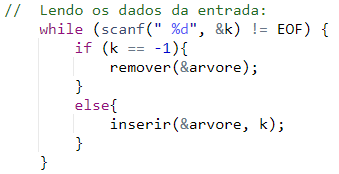
\includegraphics[width=5cm]{tudo/imagens/while_leitura.png}
    \caption{Loop \textit{while} responsável pela leitura}
    \label{imagem:leitura}
    \end{figure}

Entretanto, há mais funções que podem ser chamadas pelas próprias funções de inserção ou remoção (\textit{LeftRotate, RightRotate, ajuste}), ou chamadas de forma isolada na main, como é o caso das funções \textit{preorder}, \textit{desalocar} e \textit{busca\_no}.
\smallskip

\subsection{Inserção}
    No caso de inserção, é chamada a função \textbf{inserir} com o endereço da árvore e o número lido como parâmetros. Esta função apenas insere um número como em qualquer árvore binária. Se o número a ser inserido for menor, seguir pela esquerda, se for maior, seguir pela direita. Como a árvore é inicializada com a raiz apontando para \textit{NULL} na main, a raiz passará a apontar para o novo nó alocado, pintado de preto, sem necessidade de mais ajustes. Caso a árvore não esteja vazia, pode ser que essa inserção desbalanceie a árvore de alguma forma. Portanto, para este caso chamaremos a função de \textbf{ajuste}, que será esclarecida mais à frente. Antes de chamar a função de ajuste, será realizada a ligação do novo nó com seu pai, seus filhos apontam para \textit{NULL} e sua cor é definida como \textbf{vermelho}.
    \subsubsection{Ajuste de inserção}
        A função de \textbf{ajuste} espera como parâmetro um ponteiro do nó que acabou de ser inserido e um ponteiro para a árvore (que contém o ponteiro para a raiz em sua \textit{struct}). Agora será feita uma verificação para saber se o novo nó inserido está desbalanceando a árvore, e, caso esteja, faz as operações necessárias para tornar a árvore balanceada novamente. Para isso, será verificado, dentro de um \textit{loop}, em qual caso se encaixa o nó que estamos tratando. Neste laço há casos nos quais o problema pode ser elevado, sendo necessário fazer mais verificações. Primeiro apenas verificamos se estamos analisando a raiz, ou se o pai do nó analisado é vermelho, pois nestes caso não vamos fazer nada.

        Depois, verificaremos se estamos na sub-árvore esquerda ou direita. As operações feitas nestes dois casos são simétricas. Será criado um ponteiro apontando para o tio do nó atualmente analisado e será verificado se ele existe e se é vermelho. Caso sim, só será necessário trocar cores e depois reiniciar a análise no avô. Caso o tio não exista (\textit{NULL}) ou seja preto, vamos precisar fazer troca de cores e rotações. Será verificado se estamos no caso de rotação dupla ou simples, além de fazer as trocas de cores necessárias. Após realizar estas operações, voltamos para o \textit{while} e verificamos se precisamos fazer algo mais. Caso não, atualizamos a raiz da árvore (se necessário) e pintamos a raiz de preto, porque a raiz sempre deve ser preta.

\medskip
\subsection{Remoção}
    No caso de remoção, será chamada a função \textbf{remover}, com o endereço da árvore como argumento. Nesta função, será removido o número de menor valor da árvore binária que foi indicada como parâmetro. Primeiramente, caso a árvore exista ($raiz \neq \textit{NULL}$), seguiremos pela esquerda da árvore até achar o menor valor.

    %   Colocando figura do início da remoção
    \begin{figure}[h]
    \centering
    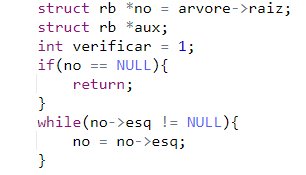
\includegraphics[width=5cm]{tudo/imagens/rm_1.png}
    \caption{Início da função de remoção, procurando pelo menor valor}
    \label{imagem:rm_1}
    \end{figure}

    Depois de encontrar o menor valor, verificaremos alguns casos básicos da remoção. O nó de menor valor pode ser a própria raiz sem filhos ou a raiz com um filho direito. No primeiro caso será necessário apenas desalocar o nó e apontar a raiz para \textit{NULL}. Se o nó for a raiz e tiver apenas o filho direito, a raiz será substituída pelo filho e pintada novamente de preto. Caso o nó não seja a raiz, ainda há dois casos que não alterarão o balanceamento da árvore. São os casos nos quais o nó é \textbf{vermelho} ou tenha um \textbf{filho da direita}. A remoção de um nó vermelho não desbalanceia a árvore, e como estamos tratando o menor valor, apenas é possível ter filho da direita. Se for este caso, o filho será colocado no lugar do nó, e sua cor será trocada. 

    %colocar imagem dos casos 0 e 1;
    \begin{figure}[h]
    \centering
    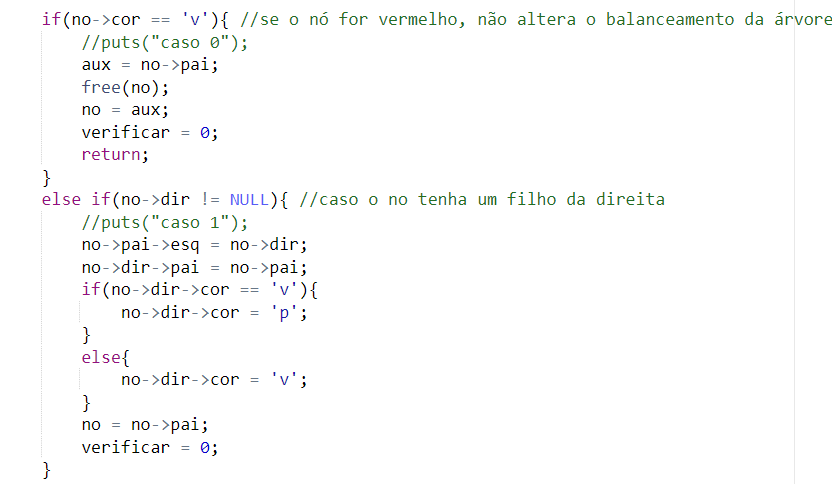
\includegraphics[width=7cm]{tudo/imagens/Casos0_1.png}
    \caption{Primeiros casos da remoção}
    \label{imagem:casos0_1}
    \end{figure}

    Porém, se não for nenhum dos casos já detalhados, entraremos em um \textit{loop} de verificação, pois podemos precisar realizar uma operação que desbalanceie outros níveis da árvore. Para entrar no \textit{while}, a variável "\textit{verificar}" deve estar com valor 1 (é atribuída como 0 se entrar em algum dos casos base) e o nó a ser verificado não pode ser a raiz (isso pode mudar dentro do \textit{loop}). Dentro deste laço, existem mais alguns casos de remoção que podemos cair. Vale lembrar que, antes de entrar, a ligação do pai com o nó que estamos tratando (o filho esquerdo) foi desfeita e o ponteiro aponta para \textit{NULL}, e todo filho \textit{NULL} é considerado como preto nas propriedades da árvore RN.
    \smallskip
    \subsubsection{Caso: Irmão Vermelho}
        Caso o irmão direito exista ($\neq$ \textit{NULL}) e ele seja vermelho, trocaremos as cores do irmão (para preto) e do pai (para vermelho), faremos uma rotação LL no pai e iremos verificar novamente. O objetivo dessas operações é fazer o nó ter um irmão preto, entrando em algum dos casos que tem esta condição (preferencialmente um que já deixe a árvore balanceada sem precisar de mais análise). Como não alteramos o valor da variável "\textit{verificar}" e também não alteramos o nó que está sendo verificado, vamos inevitavelmente passar no \textit{while} de novo.
        
    \subsubsection{Caso: Irmão preto com filho direito vermelho}
        Este é um dos casos buscados para o encerramento da análise da remoção. Quando o nó analisado tem um irmão preto com um filho direito (sobrinho distante) vermelho, podemos fazer uma troca de cor do seu pai, irmão e sobrinho, encerrando com uma rotação LL. Se o irmão do nó tiver dois filhos, este caso continua sendo o preferível, já que torna a arvore balanceada ao terminar. Portanto, neste caso mudaremos a variável de verificação para 0, possibilitando a saída do \textit{while}.
        
    \subsubsection{Caso: Irmão preto com filho esquerdo vermelho}
        Entraremos neste caso se não for possível entrar no anterior, portando aqui o nó analisado não tem o seu sobrinho distante. Neste sentido, o nosso objetivo aqui é fazer que o nó tenha um sobrinho distante vermelho, e isso é possível ao rotacionar o seu irmão com uma RR. Depois da rotação devemos atualizar as cores, e agora temos o mesmo cenário que no caso anterior, que é o sobrinho distante vermelho. Logo, repetiremos os passos e encerramos a verificação.
        
    \subsubsection{Caso: Irmão preto com filhos pretos (ou filhos \textit{NULL})}
        Entraremos neste caso se não conseguirmos entrar nos anteriores. Este caso pode ou não encerrar a análise. As cores do irmão e do pai serão trocadas. O pai receberá preto e o irmão vermelho. Se o pai, antes da troca, fosse vermelho, não será necessário verificar mais, visto que não alteramos a altura de preto da árvore. Porém, se o pai já era preto, vamos ter que manter a variável de verificação como 1 passar de novo pelo \textit{loop}, agora verificando o pai, buscando uma forma de balancear a árvore. A partir daí, podemos cair em qualquer caso, inclusive neste novamente.
        
\medskip
\subsection{Funções de rotação}
    Há no programa duas funções de rotação, que podem ser utilizadas tanto na função de inserção quanto na de remoção. As funções \textit{LeftRotate} e \textit{RightRotate} fazem as rotações LL ou RR no nó que foi passado como parâmetro. Porém, para não não ser indevidamente acessado algum local da memória, são feitas algumas verificações durante a execução dessas funções. É necessário verificar se o pai do nó chamado para a rotação é \textit{NULL}, por exemplo, visto que pode se tratar de uma rotação com a raiz.
    
    Esta função é sem retorno, logo, após atualizar os ponteiros dos nós envolvidos na rotação, o código retorna para onde foi chamada a função e continua a execução com as alterações feitas.
    
\subsection{Busca}
    Esta função recebe como parâmetro o endereço da árvore (fila de atendimento) e um número (id do cliente) para fazer uma busca e verificar se o número está ou não na árvore RN recebida e, caso seja encontrado, é retornado o ponteiro para o nó. A busca é uma busca normal para uma árvore binária. Começando na raiz, se o valor do nó é maior que o buscado, seguiremos pela direita, se for menor, seguiremos pela esquerda. Interrompemos a busca quando o valor é encontrado ou quando chegamos em um \textit{NULL}. Portanto, se o valor não for encontrado, a função retornará \textit{NULL}. Além disso, a função também imprime o resultado (se o cliente está ou não na fila de atendimento).
    
\subsection{Impressão em Pré-Ordem}
    Chamada ao final do programa, antes de desalocar a árvore, esta função imprime em Pré-Ordem toda a árvore a partir da raiz, que é recebida como parâmetro. O algoritmo é simples: primeiro se imprime o número do nó, seguido de sua cor (\textit{RED} ou \textit{BLACK}), e depois é chamada esta mesma função para seus filhos esquerdo e direito, nesta ordem.
    
\subsection{Desalocar}
    A função \textit{desalocar} serve para desalocar todos os nós de uma árvore a partir de sua raiz, que é recebida como parâmetro. É chamada ao final do código, após terminar o processo de leitura e de impressão. Os nós são desalocados como em um algoritmo em Pós-Ordem, ou seja, primeiro chamamos a função de forma recursiva para os filhos da esquerda até chegar a NULL, depois os da direita, e a última instrução é de \textit{free} (desalocar o conteúdo do ponteiro).
    
\bigskip
\section{Testes}
    Depois da implementação do código na linguagem de programação C, foram realizados vários testes com o objetivo de saber como o programa se comporta ao aumentar a quantidade de clientes na lista de atendimento. Os testes da imagem \ref{imagem:grafico} foram feitos com o caso inicial de 100000 (cem mil) inserções, aumentando 50000 (cinquenta mil) a cada teste até chegar à 1000000 (um milhão) de entradas. Cada teste foi feito 7 vezes com a mesma quantidade de entrada, e o tempo final (em segundos) inserido no gráfico é um tempo médio desses 7 testes. 
    
    %Gráfico dos testes;
    \begin{figure}[h]
    \centering
    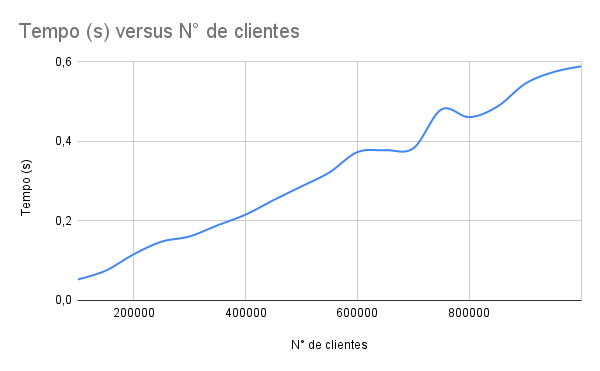
\includegraphics[width=10cm]{tudo/imagens/Tempo (s) versus N° de clientes.png}
    \caption{Gráfico relacionando a quantidade de clientes com o tempo de execução}
    \label{imagem:grafico}
    \end{figure}
    
\section{Conclusão}
    Após a análise do resultado dos testes, podemos perceber que estrutura de dados árvore Rubro Negra possibilita um programa extremamente eficiente para a implementação da fila de atendimento, visto que mesmo com uma grande quantidade de entradas, a construção da árvore demora menos de um segundo para ser feita. Portanto, considerando esta rapidez do algoritmo, podemos concluir que a árvore Rubro Negra, com todas as suas propriedades de balanceamento e formas de inserção e remoção, é uma ótima estrutura de dados para este tipo de aplicação.
    
\bigskip
\section{Referências}
    \begin{enumerate}
        \item Cormen, T. H. (2009). \textit{Algoritmos: Teoria e prática}. Elsevier Editora Ltda., Rua Sete de Setembro, 111, 16º andar.
    
        \item Szwarcfiter, J. L. e Markenzon, L. (2013) \textit{Estruturas de Dados e seus Algoritmos}. Editora LTC.
    
        \item Wirth, N. (1999). \textit{Algoritmos e estruturas de dados}. Editora LTC, Rio de Janeiro.
    \end{enumerate}

\end{document}
